\documentclass[xcolor={dvipsnames}]{beamer}

\usetheme{Malmoe}
\usecolortheme{seagull}
\usepackage[]{natbib}
\usepackage{textpos}
\usepackage{amsmath, amssymb, bm}
\usepackage{multirow}
\usepackage{framed}
\usepackage{schemata}
\setbeamertemplate{navigation symbols}{}
\usepackage[english]{babel}
\usepackage{graphics}
\usepackage{fontawesome}
\usepackage{xcolor}
\usepackage[export]{adjustbox}
\usepackage{tikz,graphicx,animate}

\definecolor{lightpink2}{rgb}{0.145,0.6666,1} % Defines the color used for content box headers
\definecolor{Red}{rgb}{0.9,0.15,0}
\definecolor{pink2}{RGB}{55,126,184}
\definecolor{Green}{RGB}{77,175,74}
\definecolor{White}{RGB}{255,255,255}
\definecolor{Lightgray}{rgb}{0.86,0.86,0.86}
\definecolor{pink2}{rgb}{1.0, 0.33, 0.64}
\definecolor{blue2}{rgb}{0.0, 0.53, 0.74}
%\definecolor{Mycolor1}{HTML}{CABED0}
%\definecolor{Mycolor9}{HTML}{3F2949}

\setbeamertemplate{footline}
{
	\leavevmode%
	\hbox{%
		\begin{beamercolorbox}[wd=.50\paperwidth,ht=2.25ex,dp=1ex,center]{author in head/foot}%
			\usebeamerfont{author in head/foot}\insertshortauthor%% \beamer@ifempty{\insertshortinstitute}{}{(\insertshortinstitute)}
		\end{beamercolorbox}%
%		\hskip2pt%
		\begin{beamercolorbox}[wd=.50\paperwidth,ht=2.25ex,dp=1ex,center]{title in head/foot}%
			\usebeamerfont{title in head/foot}\insertshorttitle~~~~~~~~~~~~~~~~~~~~~~~~~~\insertframenumber
		\end{beamercolorbox}%
	}%
	\vskip0pt%
}
\makeatother

\title[Demography matters]{}

\subtitle{\Large{\textbf{Life expectancy changes during the pandemic in low mortality countries}}}

\author[CPC Seminar 2021]
{
	\vspace{-0.5cm}
	\texorpdfstring{
		\begin{columns}
			\column{.9\linewidth}
			\centering
								$\,$\\
			\Large{\textbf{Jos\'{e} Manuel Aburto}}\\				
			\faTwitter \quad  @jm\_aburto \\
			$\,$\\

\includegraphics[width=1.15\textwidth,center]{Figures/logos}\\
		\end{columns}
	}
	{}
}
\date{}

\beamertemplatenavigationsymbolsempty
\begin{document}


\begin{frame}[plain]
	\titlepage
\end{frame}
%%%%%%%%%%%%%%%%%%%%%%%%%%%%%%%%%%%%%%%%%%%%%%%%%%%%%%%%%%%%%%%%%%%%%%%%%
%%%%%%%%%%%%%%%%%%%%%%%%%%%%%%%%%%%%%%%%%%%%%%%%%%%%%%%%%%%%%%%%%%%%%%%%%


%%%%%%%%%%%%%%%%%%%%%%%%%%%%%%%%%%%%%%%%%%%%%%%%%%%%%%%%%%%%%%%%%%%%%%%%%
\begin{frame}
	\begin{center}
	
		\LARGE{\textbf{Demography as a discipline to study structural social 				changes}}
		
	\end{center}
\end{frame}



\begin{frame}
	\begin{center}
		\LARGE{\textbf{Demography during the COVID-19 pandemic}}\linebreak 
		
		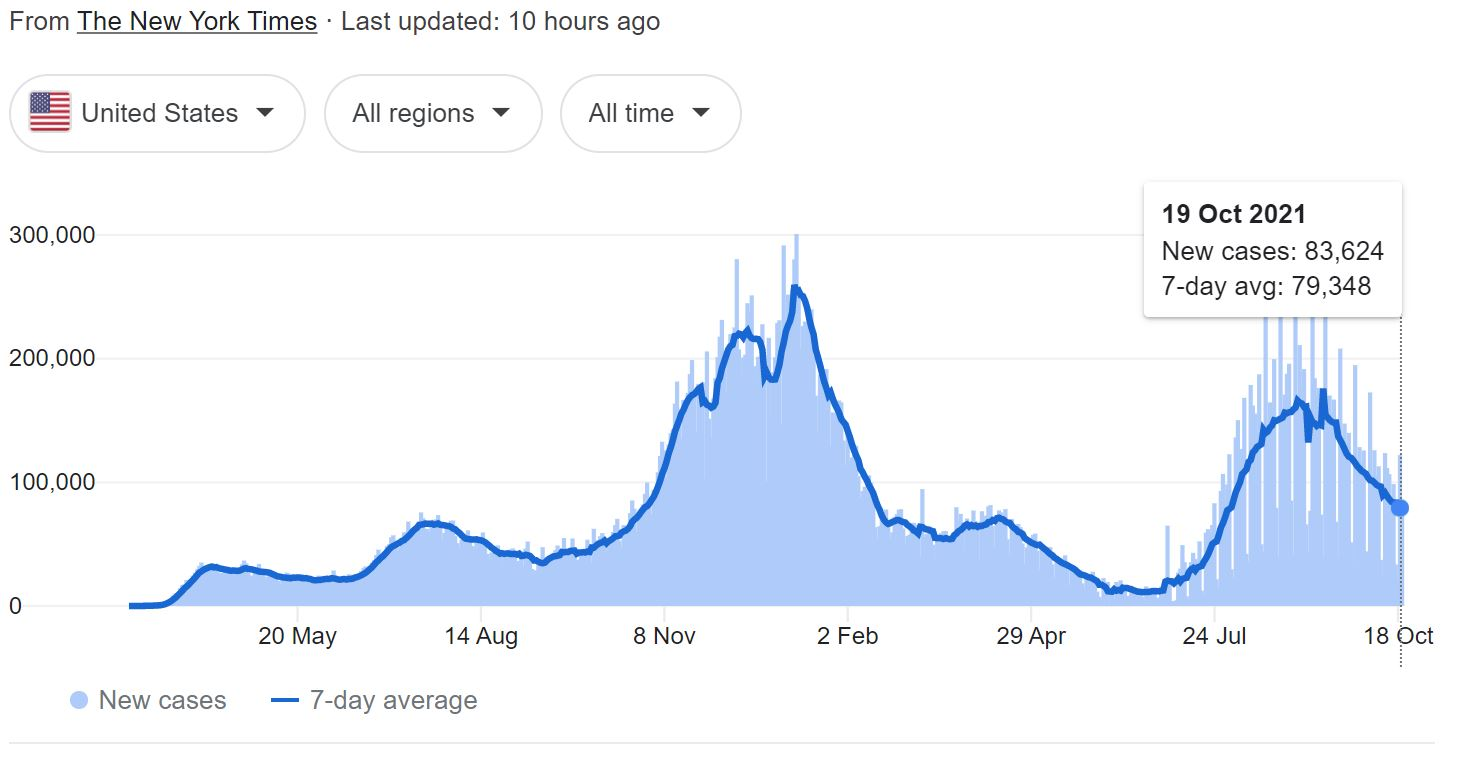
\includegraphics[scale=.25]{Figures/covid19}
		
		\pause
		
		\Large{From Ronald Lee's \textit{Demography abandons its core}:  Formal 			demography is in a coma. Perhaps we should just let it die a natural 				death.}
		
	\end{center}
\end{frame}

\begin{frame}
	\begin{center}
		\LARGE{\textbf{Excess deaths}}			
		
		\begin{columns}
			\begin{column}{0.73\textwidth}
				\begin{tikzpicture}
					\node (img) {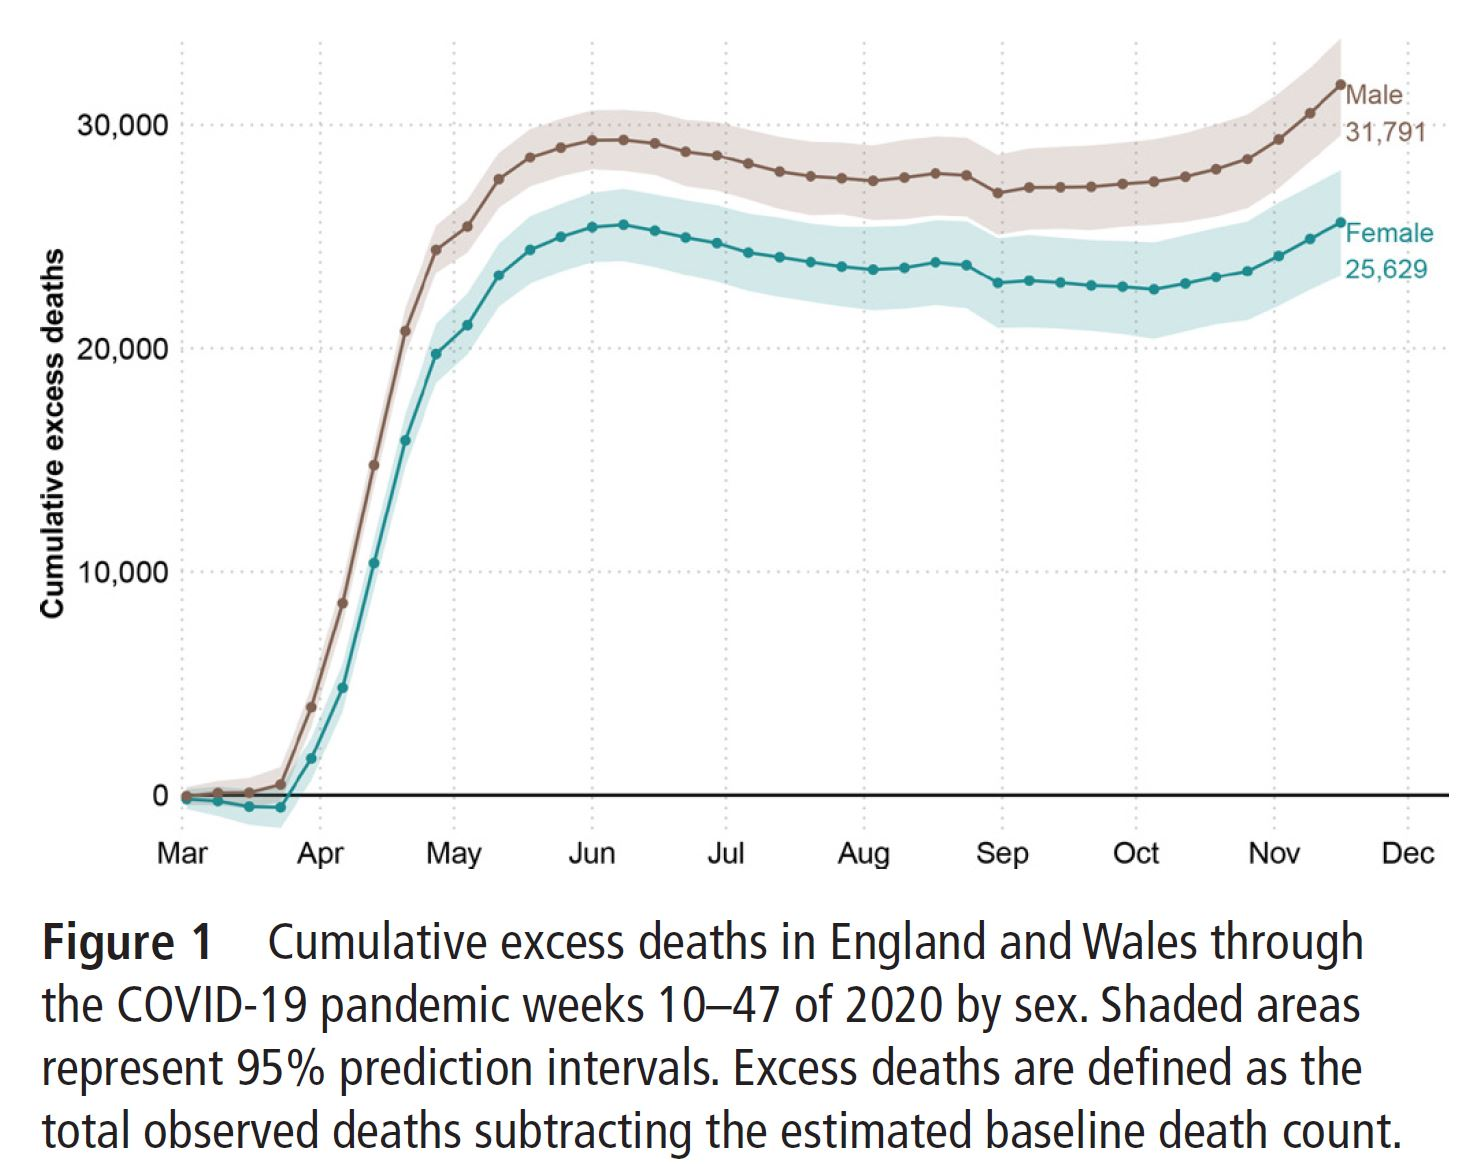
\includegraphics[width=1.2\textwidth]{Figures/Excess_England}};
				\end{tikzpicture}
			\end{column}
	
			\begin{column}{0.25\textwidth}
				\begin{tikzpicture}
				\node (img){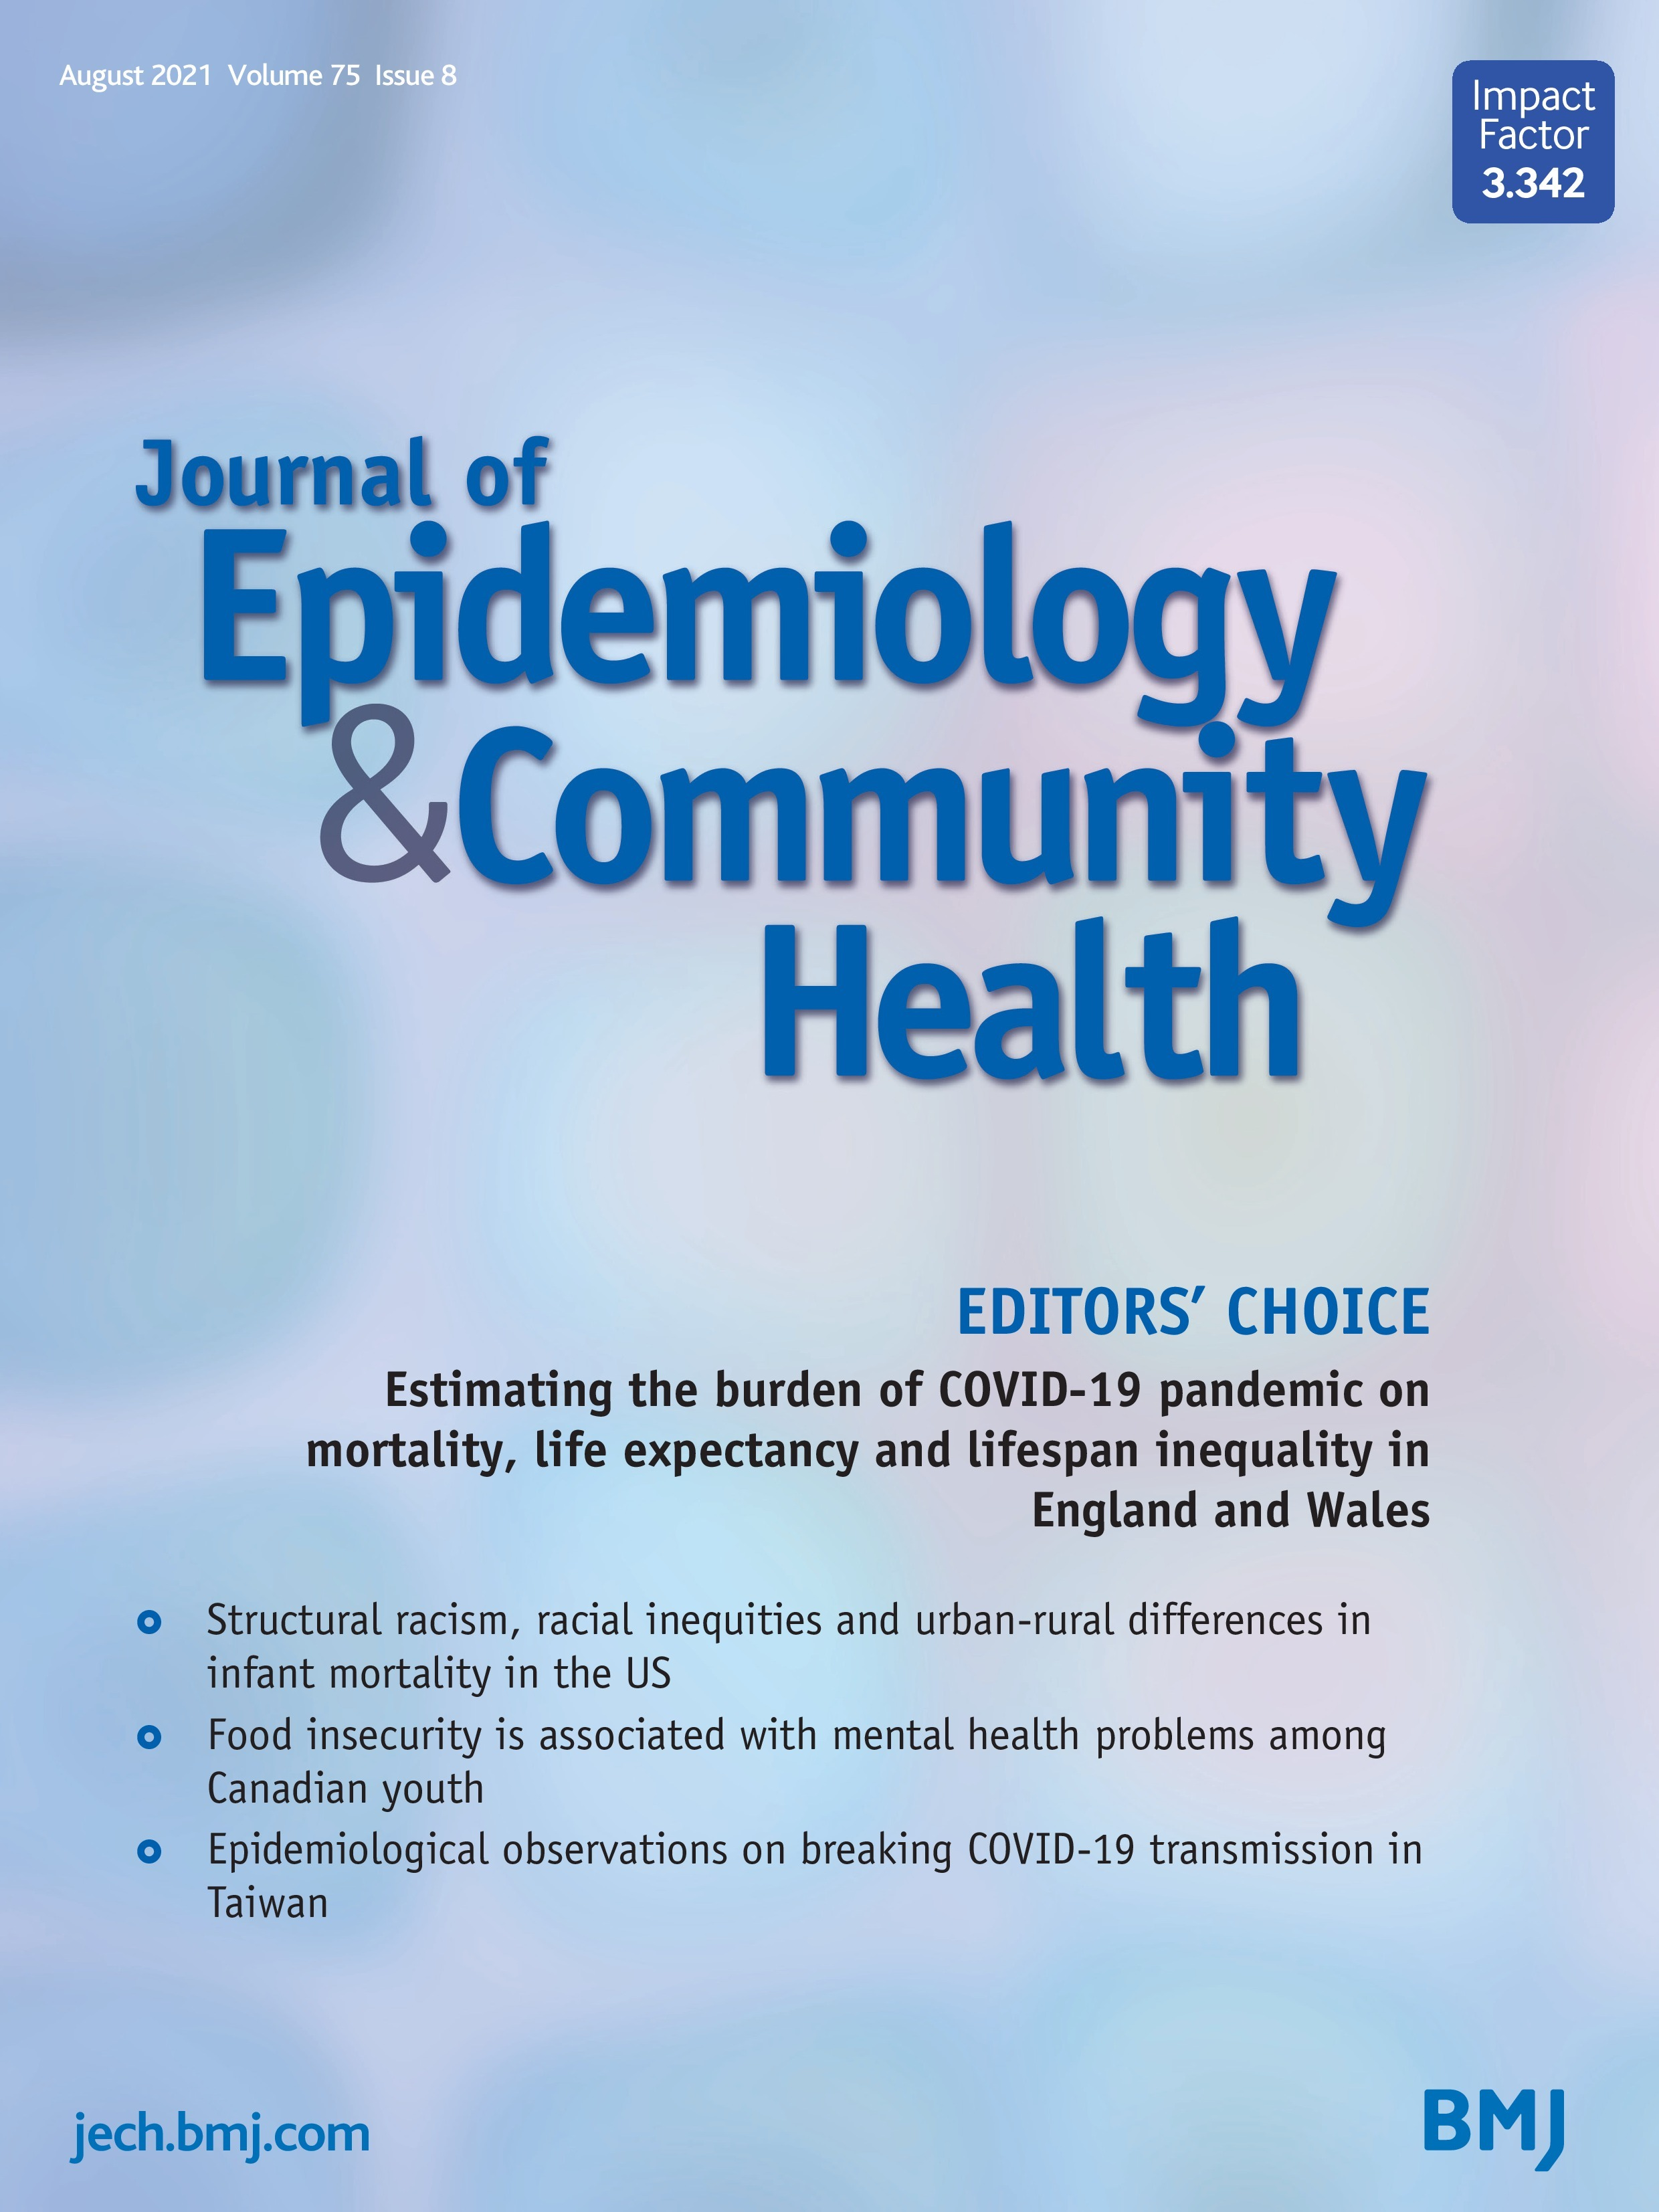
\includegraphics[width=.9\textwidth]{Figures/England_paper}};
				\end{tikzpicture}
			\end{column}
		\end{columns}
	\end{center}

\tiny{Aburto et al 2021, Journal of Epidemiology and Community Health}
		
\end{frame}


\begin{frame}
	\begin{center}
		\LARGE{\textbf{Excess deaths by age}}			
		
				\begin{tikzpicture}
					\node (img) {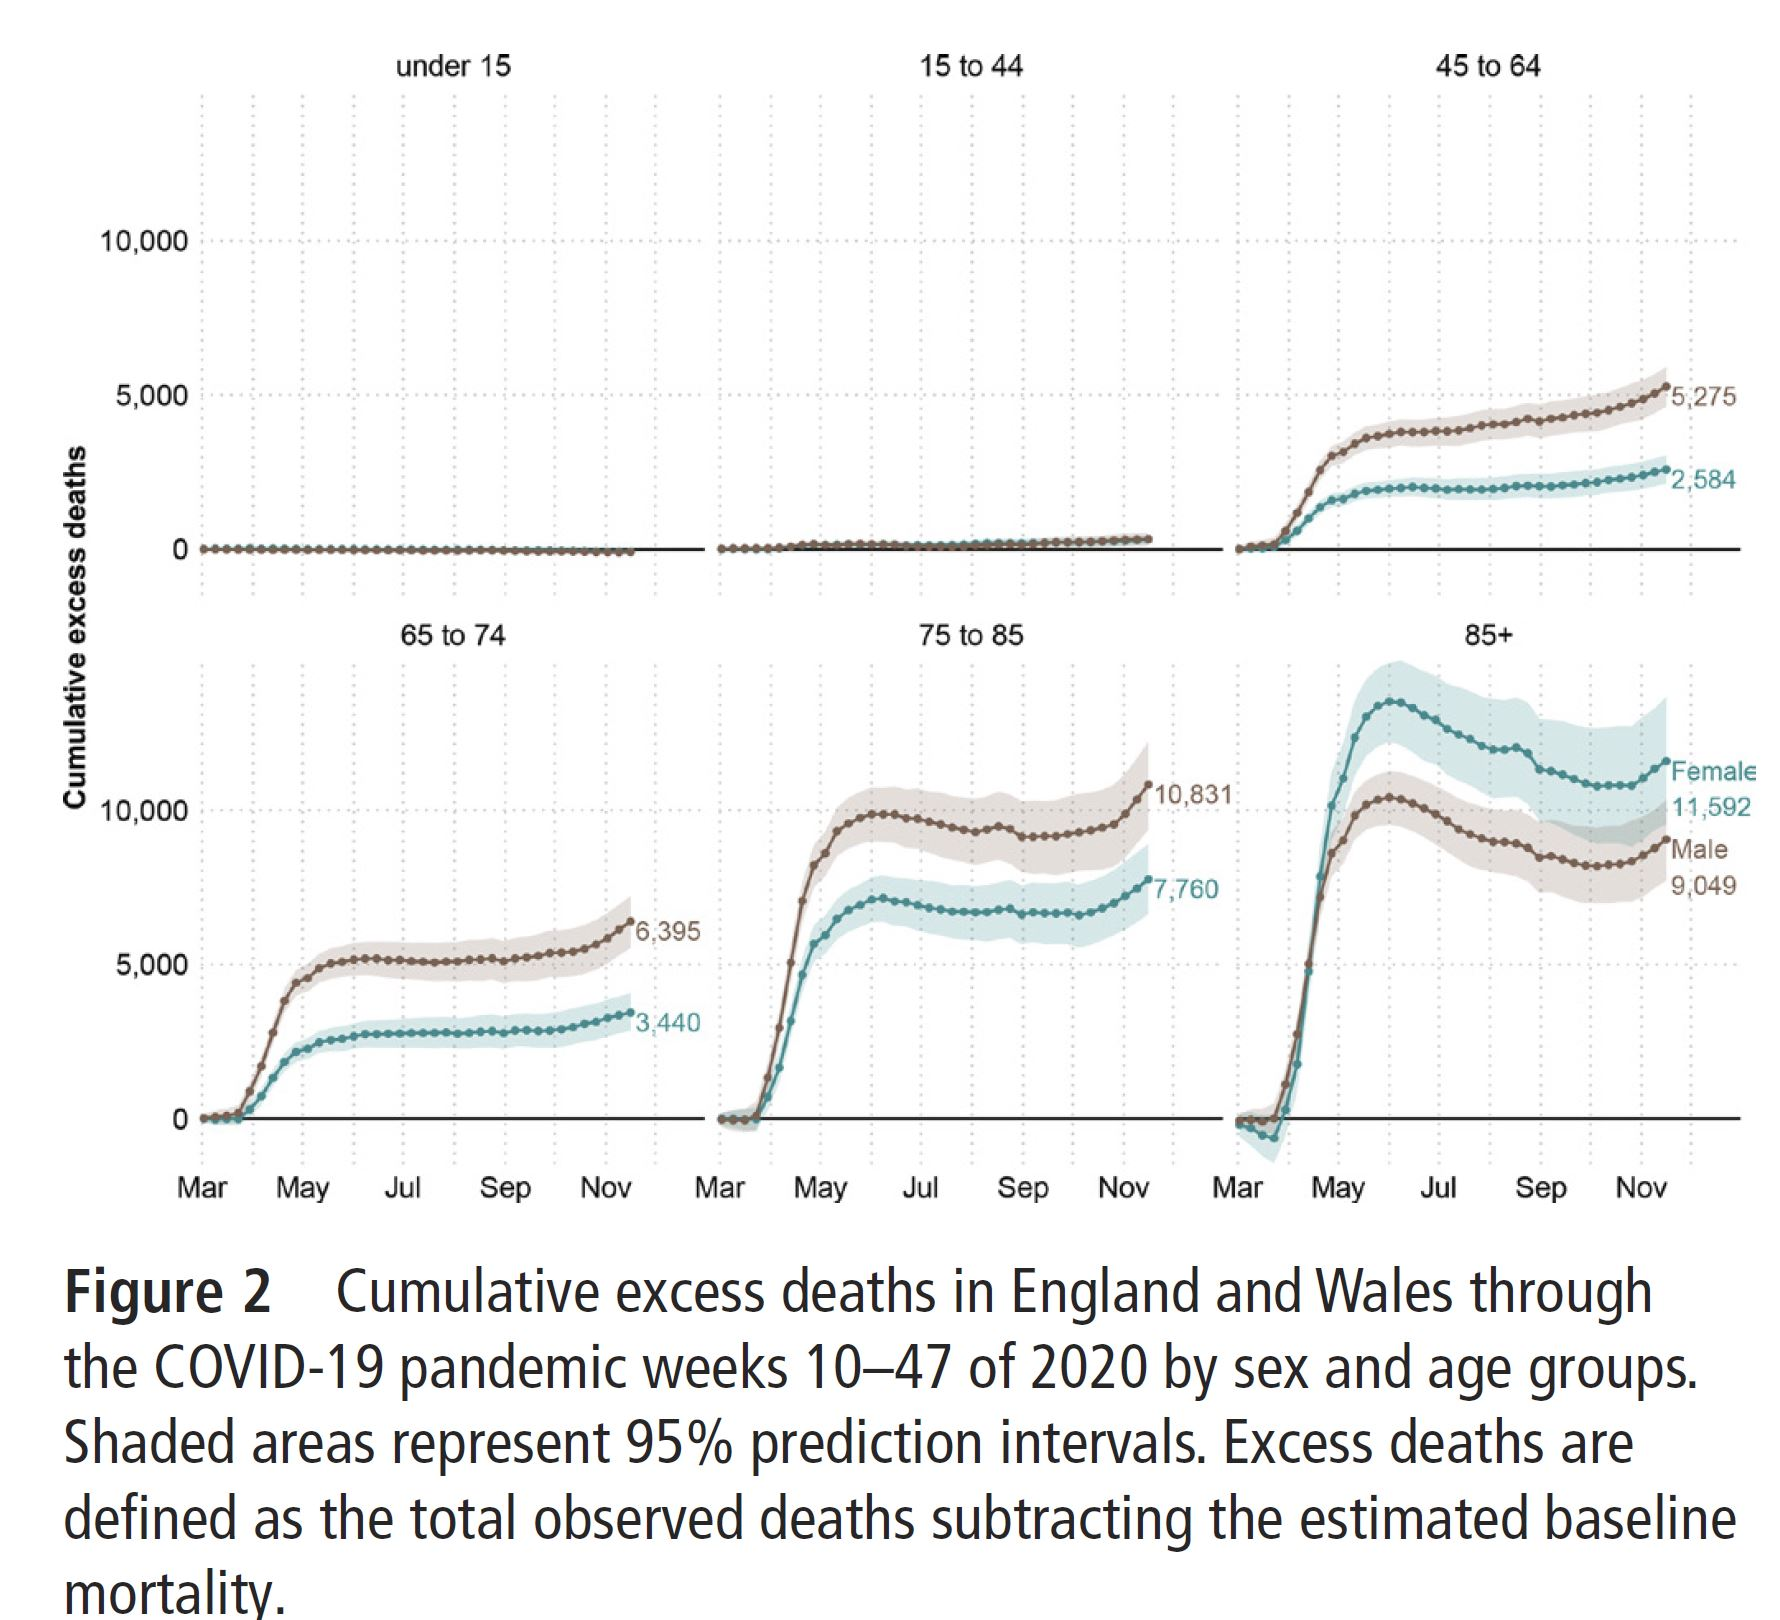
\includegraphics[width=.75\textwidth]{Figures/Excess_England_2}};
				\end{tikzpicture}

	\end{center}

\tiny{Aburto et al 2021, Journal of Epidemiology and Community Health}
		
\end{frame}



\begin{frame}
	\begin{center}
		\LARGE{\textbf{Excess deaths overcome some limitations:}\linebreak 
		
		\begin{itemize}
			\item \textcolor{gray}{Different testing strategies.}
			\item \textcolor{gray}{Coding practices.}
			\item \textcolor{gray}{Potential undercounting.}
			\item \textcolor{gray}{Accounts for population age-structure.}
			\item \textcolor{gray}{Accounts for population change.} \linebreak
		\end{itemize} 
		
		\pause
		
		\textbf{BUT, it is very difficult to make comparisons.}
		
		}
	\end{center}
\end{frame}

\begin{frame}
	\begin{center}
		\LARGE{\textbf{Demographer's perspective}} \linebreak
		
\Large{\textcolor{darkgray}{We need to go beyond excess deaths and country-specific analyses and focus on the pressing issue of revealing the impacts of the pandemic on life expectancy in a cross-national perspective.}}
	\end{center}			
\end{frame}


\begin{frame}
	\begin{center}
		\LARGE{\textbf{What is life expectancy?}} \pause \linebreak
	
\Large{\textcolor{darkgray}{Average number of years a \textbf{synthetic} cohort of newborns would live if they were to experience the death rates observed in a given period throughout their lifespan}} 

	\end{center}
			
\end{frame}


\begin{frame}
	\begin{center}
		\LARGE{\textbf{Why life expectancy?}} \pause \linebreak
	
	\end{center}
		\begin{itemize}
	\Large{
	\item \textcolor{gray}{Widely used metric of population health.}
	\item \textcolor{gray}{Comparable across countries and over time.}
	\item \textcolor{gray}{Summarizes mortality in a given year.}
	\item \textcolor{gray}{Decomposable with demographic methods.}
	}
	\end{itemize}
\end{frame}


\begin{frame}
	\begin{center}
		\LARGE{\textbf{Challenges for timely life expectancy estimates}} \pause \linebreak
	
	\end{center}
		\begin{itemize}
	\Large{
	\item \textcolor{gray}{Timely all-cause mortality data.}
	\item \textcolor{gray}{High quality coverage.}
	\item \textcolor{gray}{Disaggregates by age and sex (minimum).}
	\item \textcolor{gray}{Population estimates.}
	}
	\end{itemize}
\end{frame}


\begin{frame}
	\Large{	
	\begin{center}
		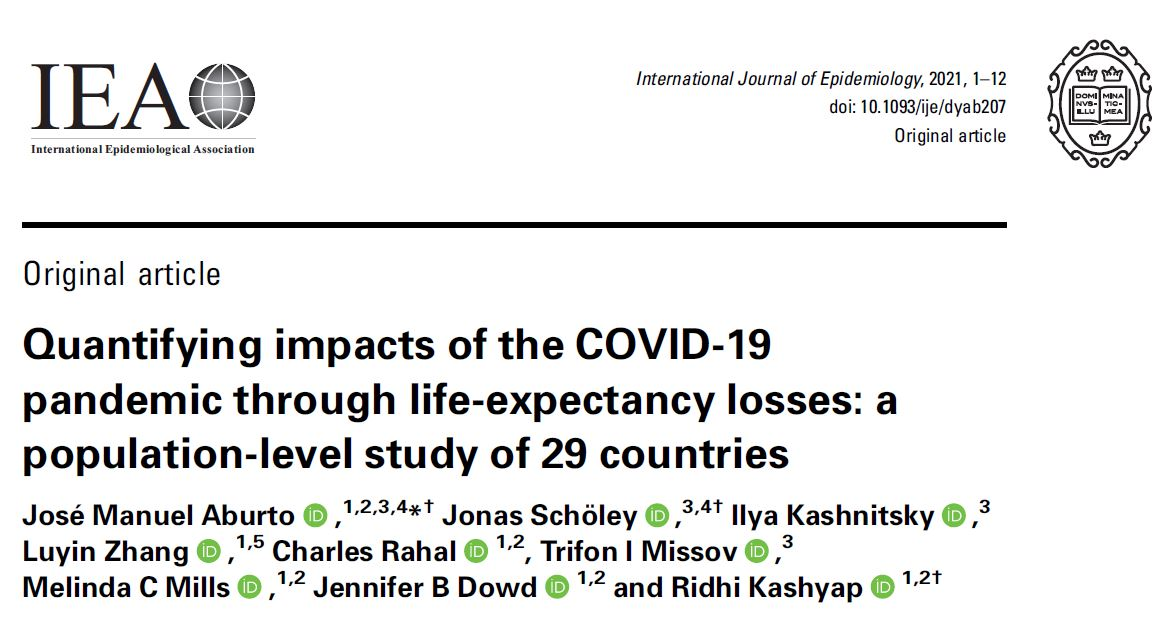
\includegraphics[scale=.45]{Figures/IJE_Aburto}
		
	\end{center}
		}
\end{frame}


\begin{frame}
\begin{center}

 \begin{tikzpicture}
\node (img) {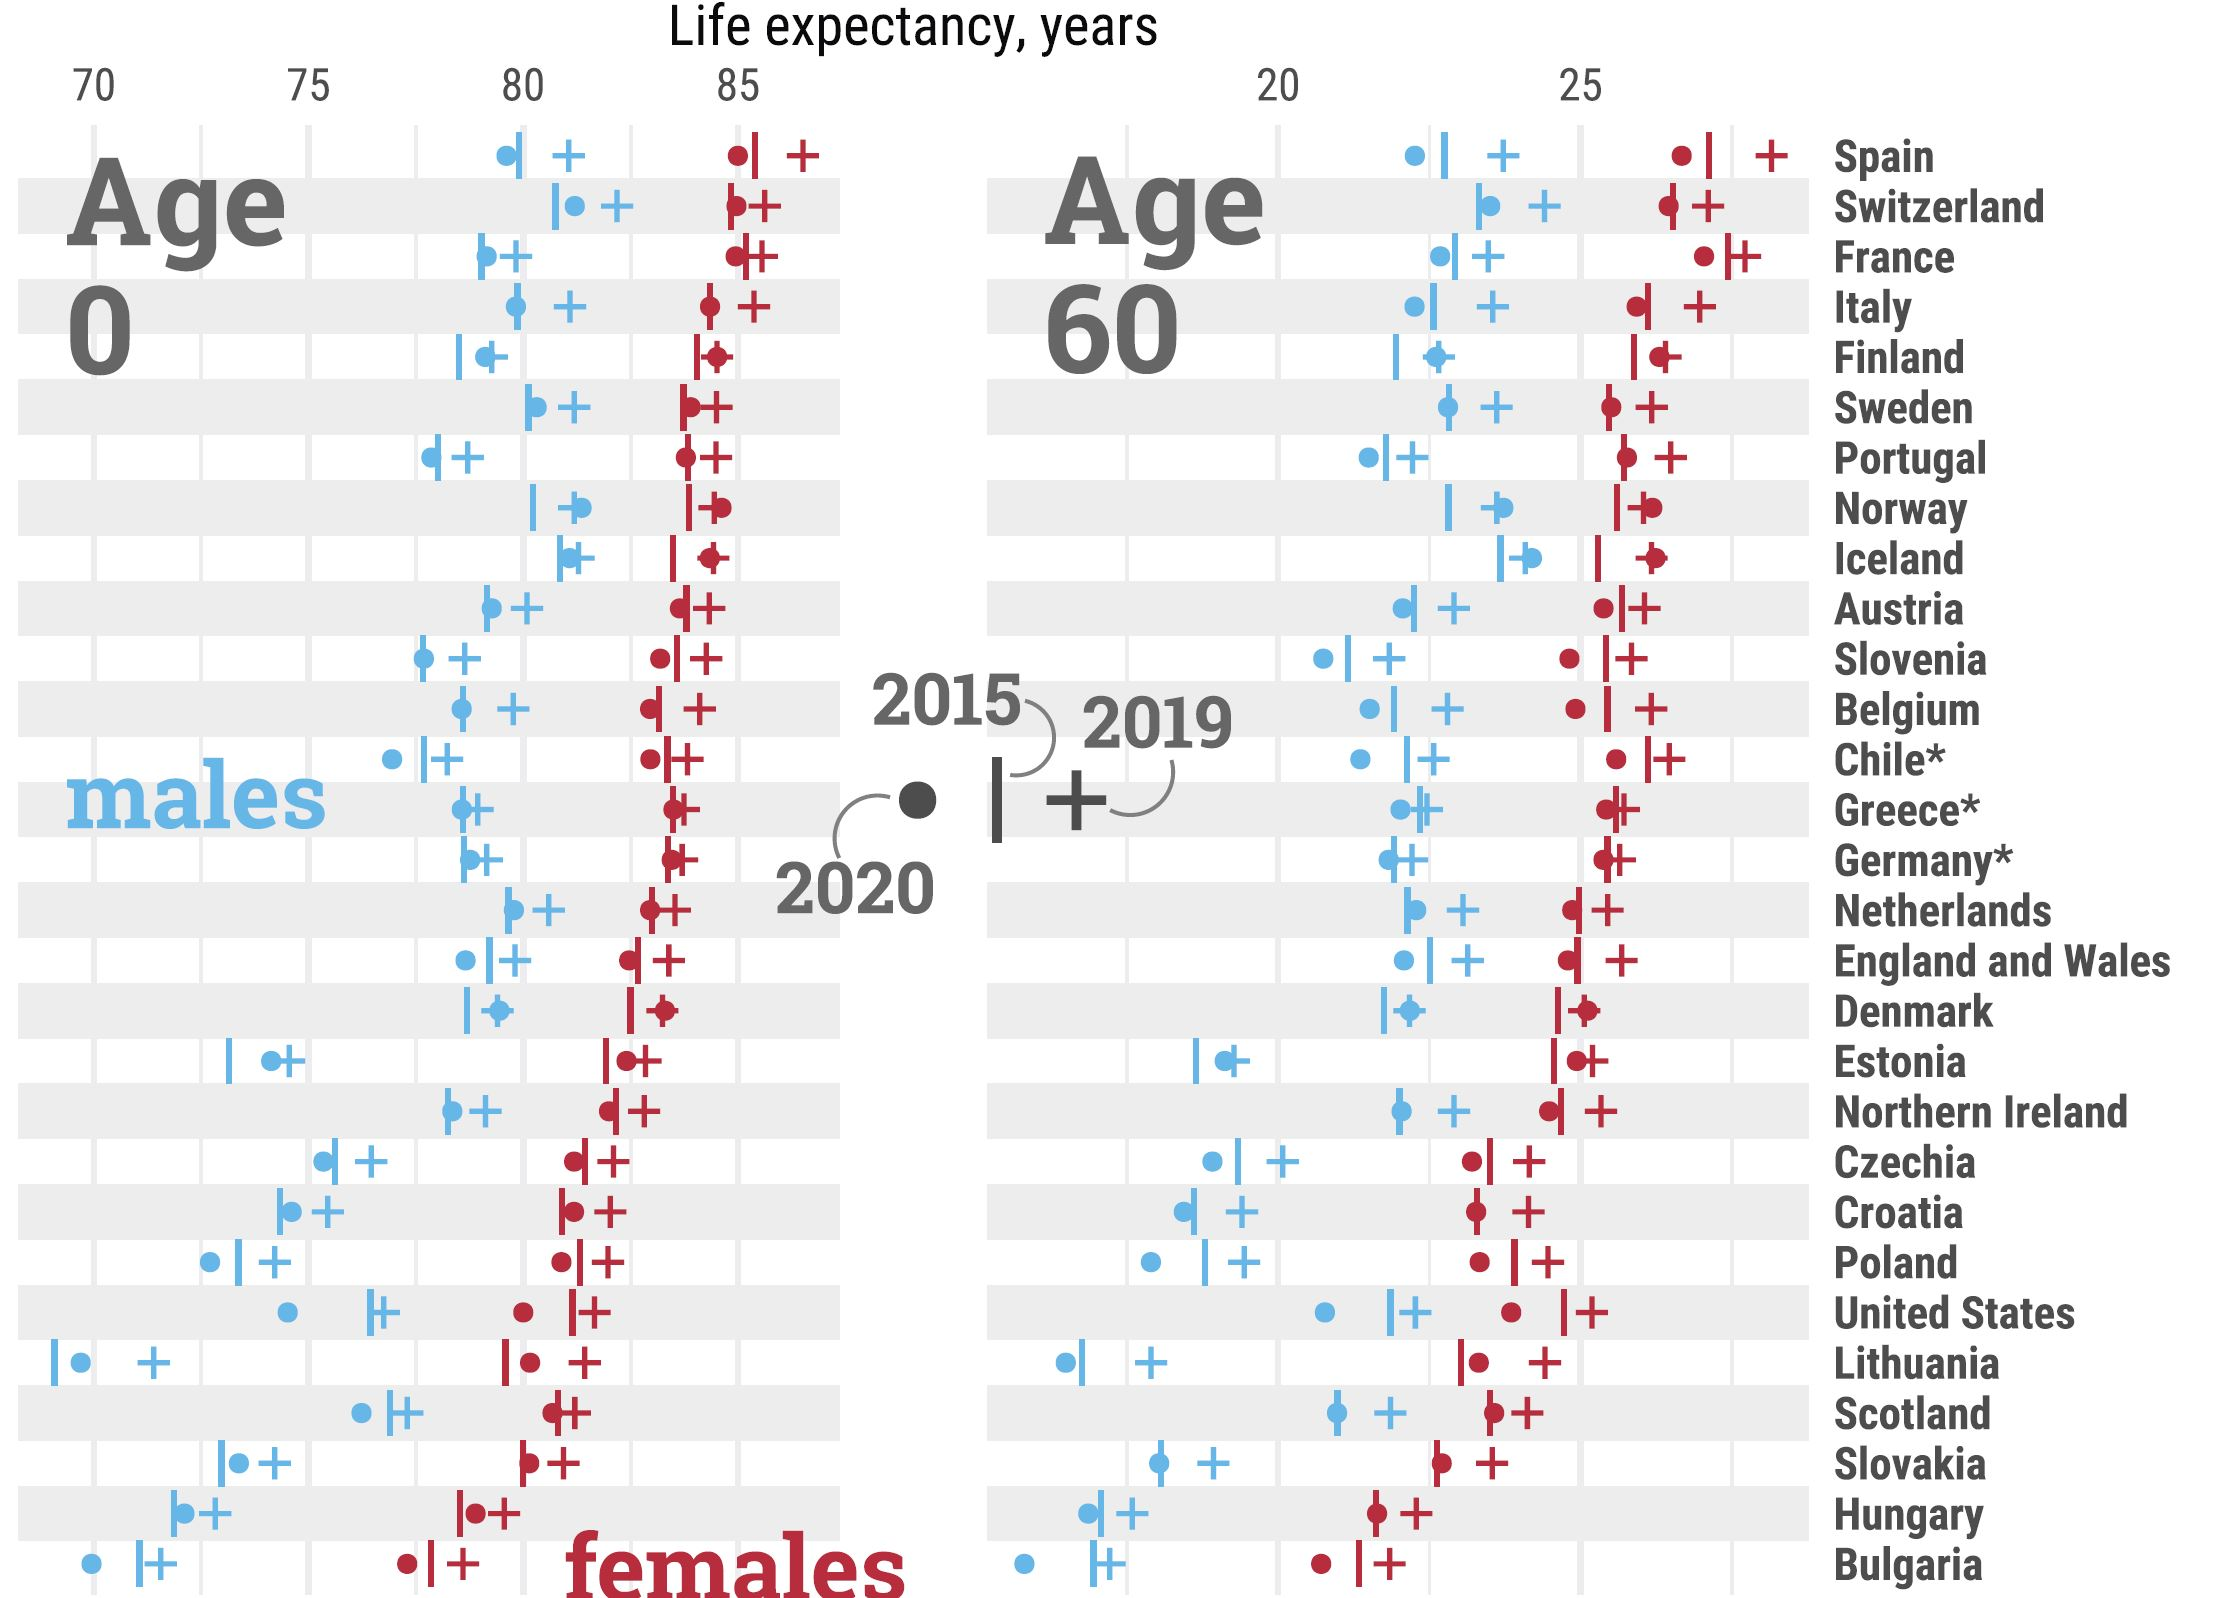
\includegraphics[width=1.07\textwidth]{Figures/IJE_1}};
\end{tikzpicture}

\end{center}
\end{frame}

\begin{frame}
\begin{center}

 \begin{tikzpicture}
\node (img) {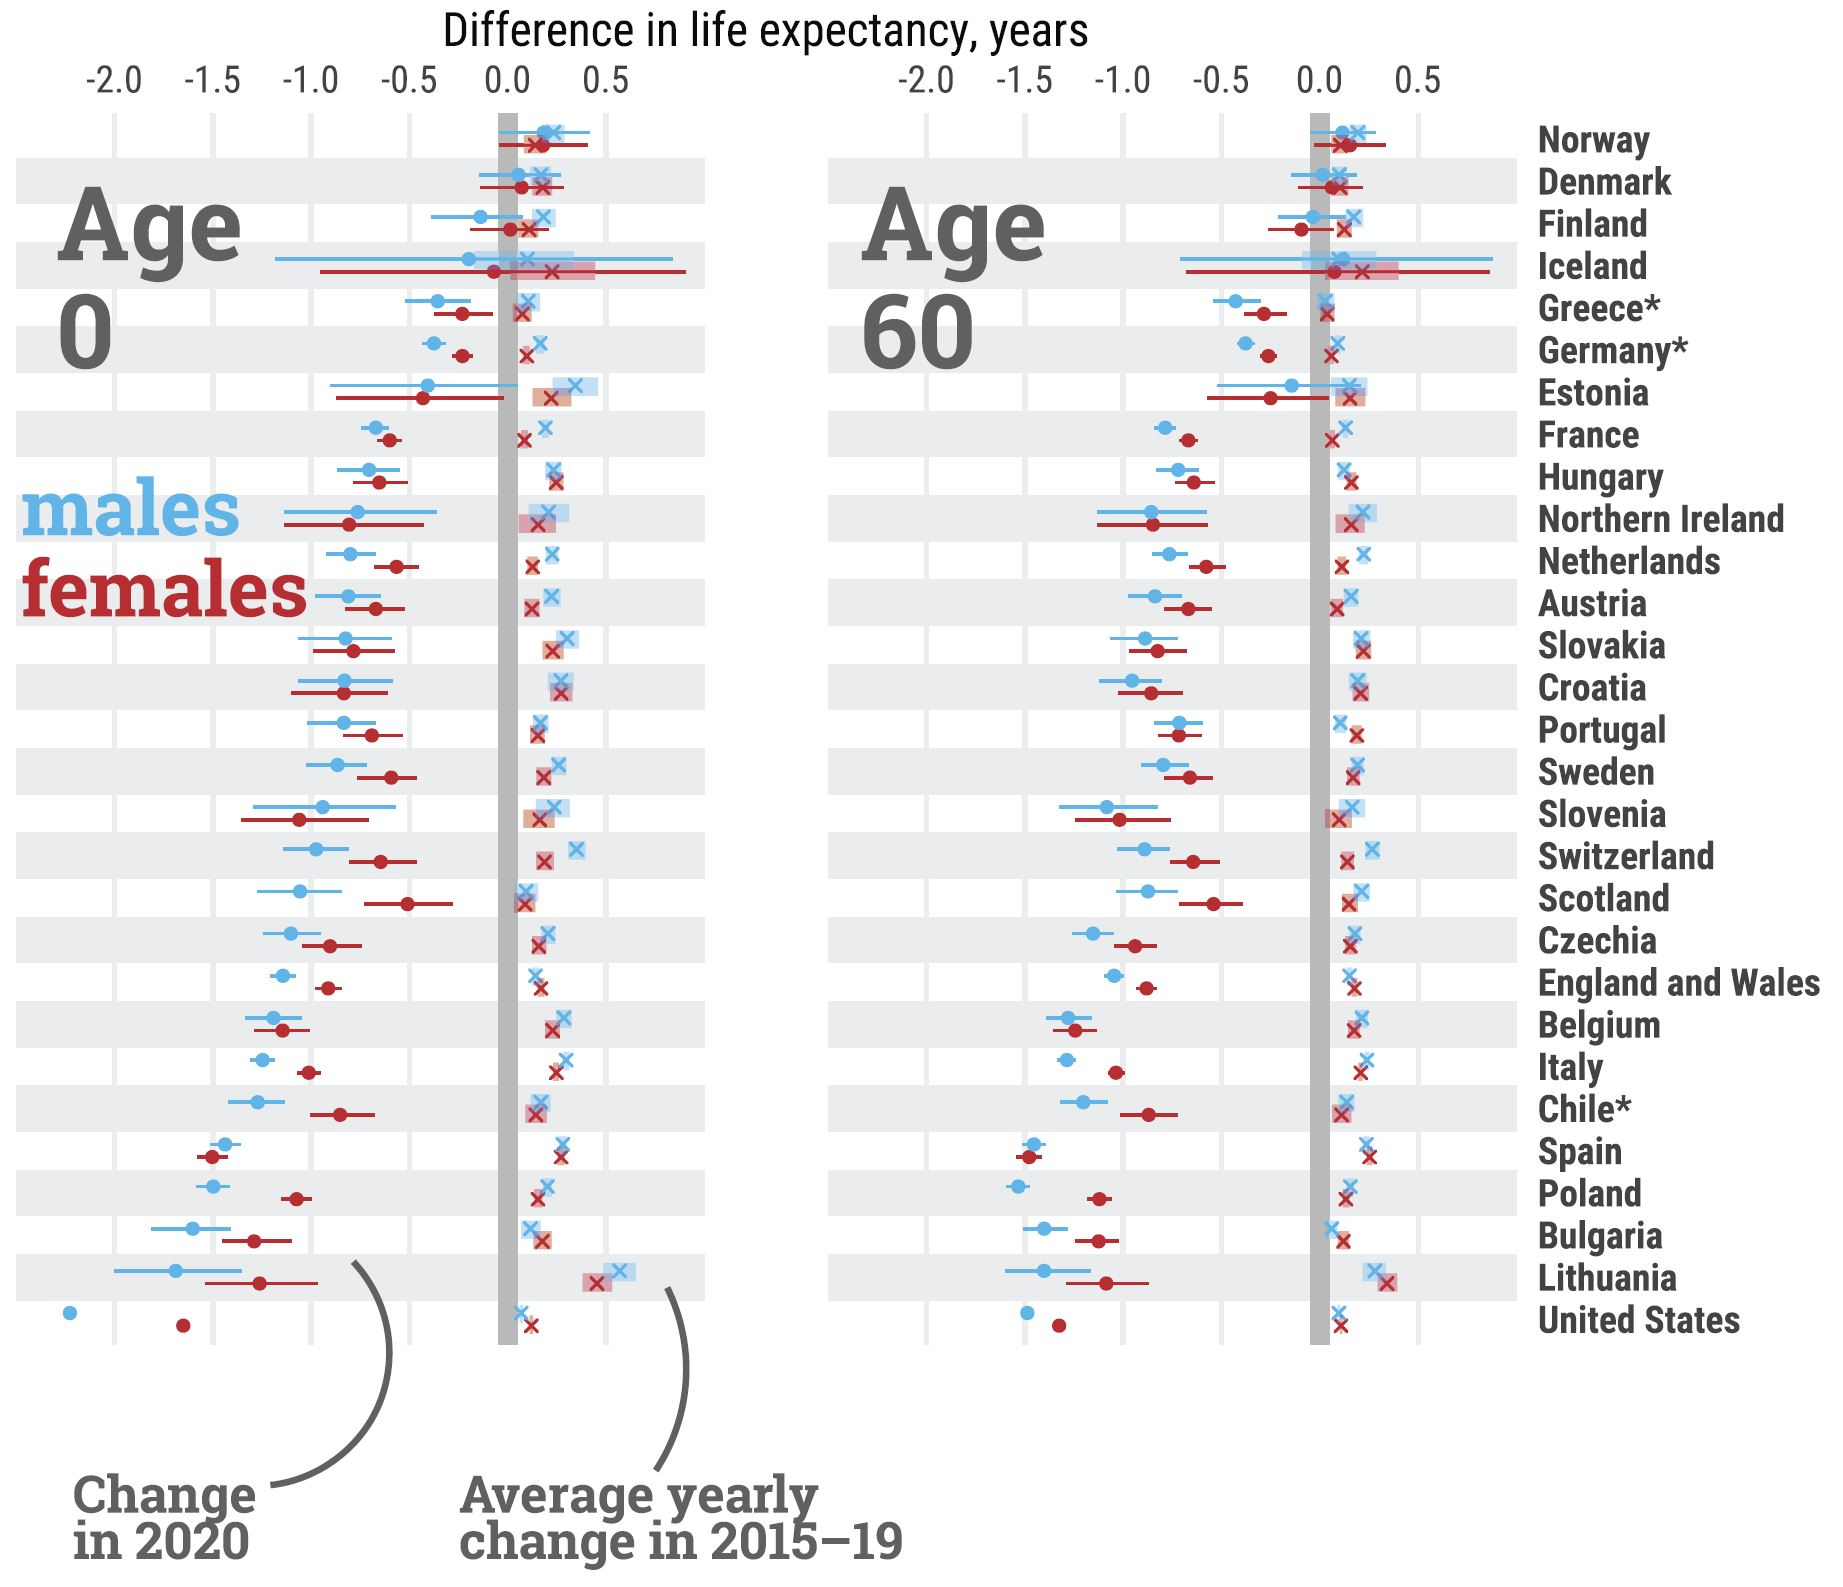
\includegraphics[width=.97\textwidth]{Figures/IJE_2}};
\end{tikzpicture}

\end{center}
\end{frame}


\begin{frame}
\begin{center}

 \LARGE{\textbf{Historical context}}
 
 	\animategraphics[height=2.5in,controls = play]{15}{imgpdf/animate_}{0}{299}
												

\end{center}
\end{frame}


\begin{frame}
\begin{center}

 \LARGE{\textbf{Age-specific contributions}}
\hspace*{-1cm}
 \begin{tikzpicture}
\node (img) {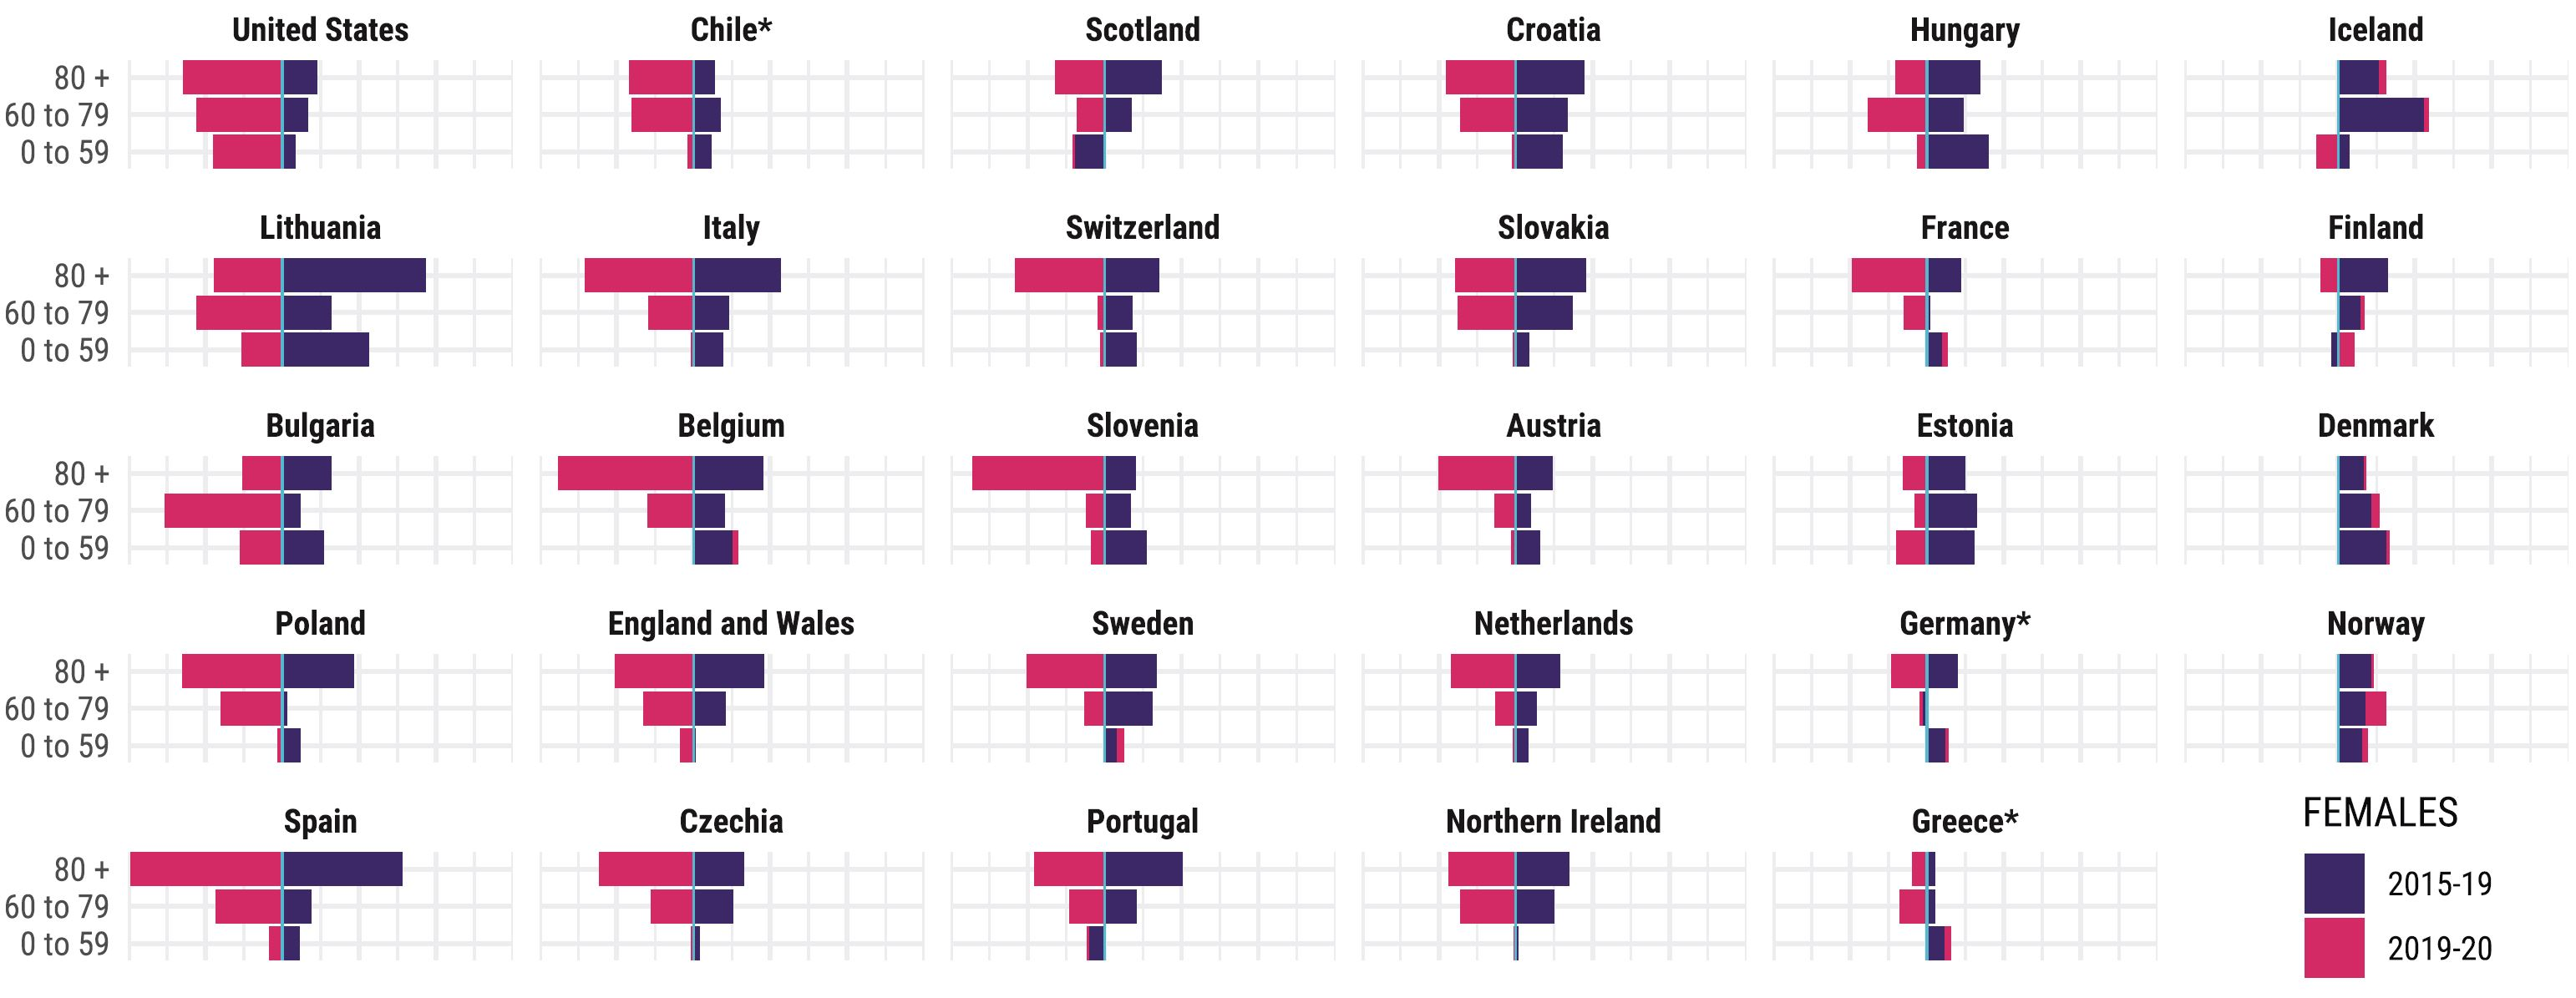
\includegraphics[width=1.13\textwidth]{Figures/IJE_3}};
\end{tikzpicture}

\end{center}
\end{frame}

\begin{frame}
\begin{center}

 \LARGE{\textbf{Age-specific contributions}}
\hspace*{-1cm}
 \begin{tikzpicture}
\node (img) {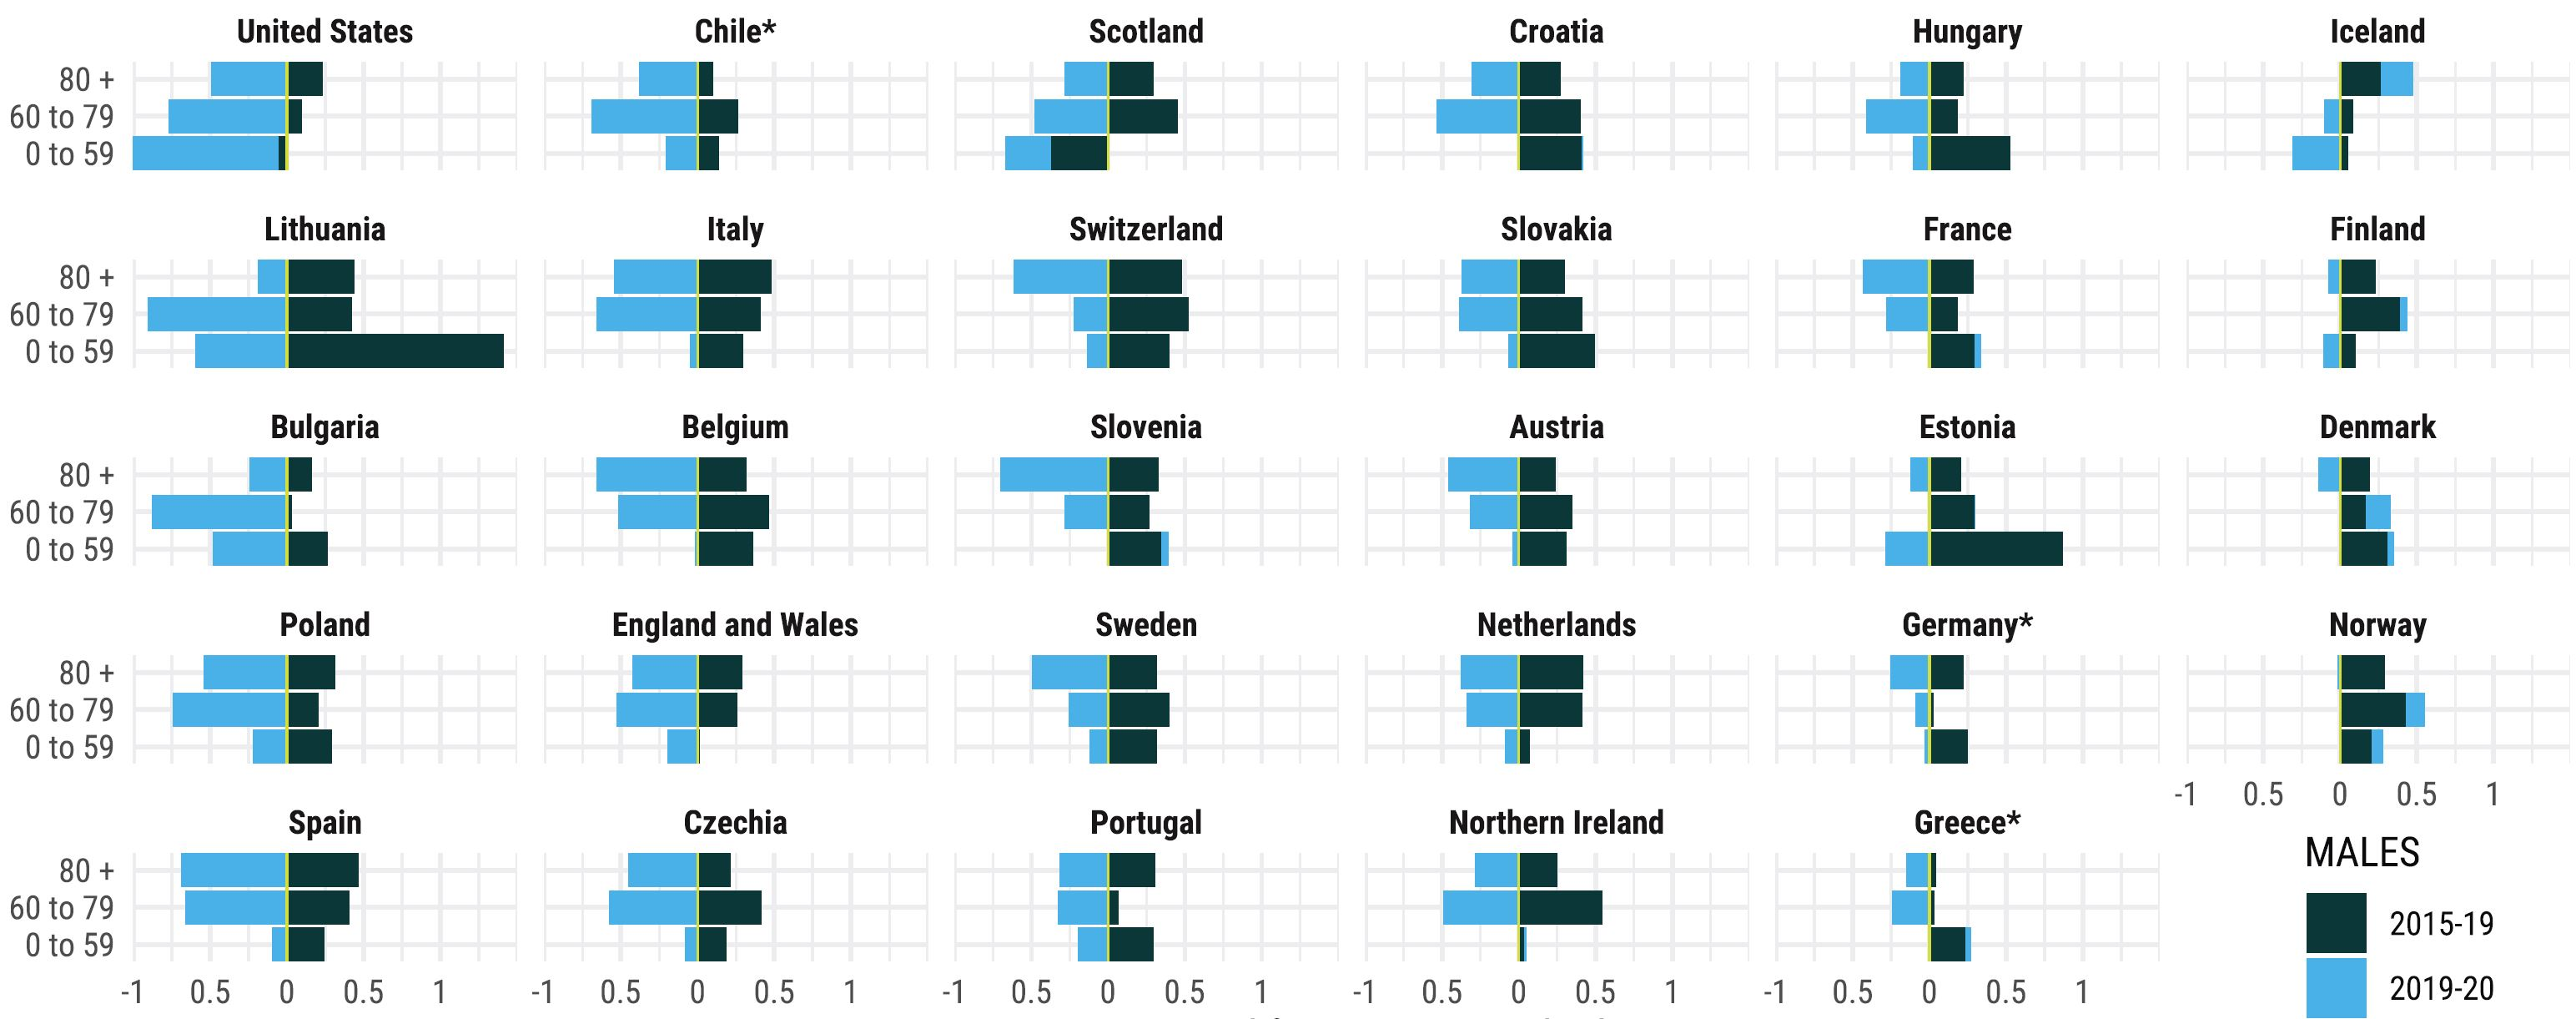
\includegraphics[width=1.13\textwidth]{Figures/IJE_4}};
\end{tikzpicture}

\end{center}
\end{frame}


\begin{frame}
\begin{center}
 \LARGE{\textbf{COVID-19 contribution}}
\end{center}


 \begin{tikzpicture}
\node (img) {\hspace*{0.5cm}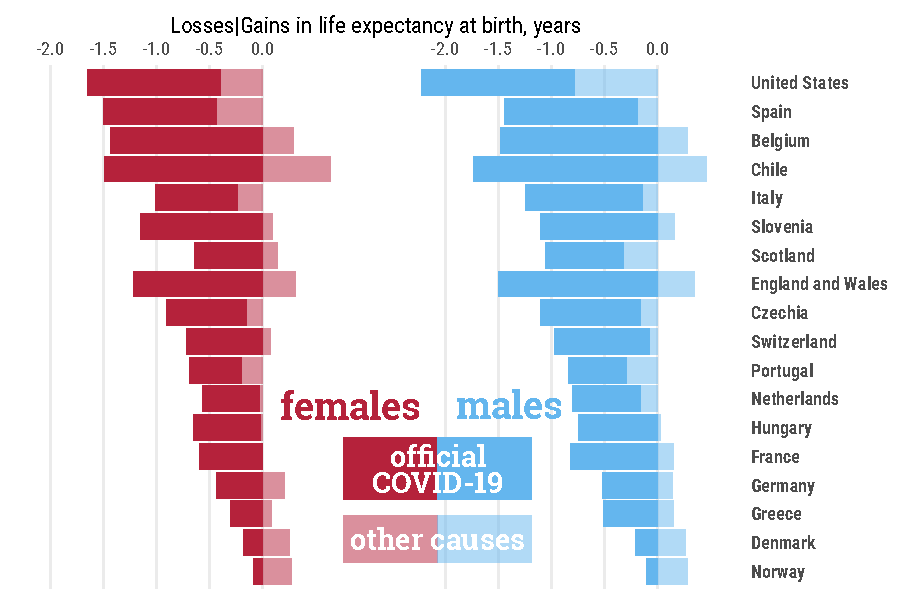
\includegraphics[width=1\textwidth]{Figures/fig 5_final}};
\end{tikzpicture}

\end{frame}

\begin{frame}
	\begin{center}
 		\LARGE{\textbf{Key points}}
 		\Large{
 		\begin{itemize}
 		\item Out of 29 countries analysed, 27 had losses. \pause
 		\item 11 countries for males and 8 among females  $>1$ year. \pause
 		\item Females from 15 countries and males from 10 ended up with lower life expectancy at birth in 2020 than in 2015.\pause
 		\item Losses in life expectancy were largely attributable to increased mortality above age 60 years and linked to official COVID-19 deaths.

 		\end{itemize}
 		}
	\end{center}
\end{frame}



\begin{frame}
	\begin{center}
	
			\LARGE{\textbf{Sex differences: males tend to have greater losses than 				females.}\linebreak \\ \pause
			
			But not everywhere}
		
	\end{center}
\end{frame}


\begin{frame}
	\begin{center}
	
		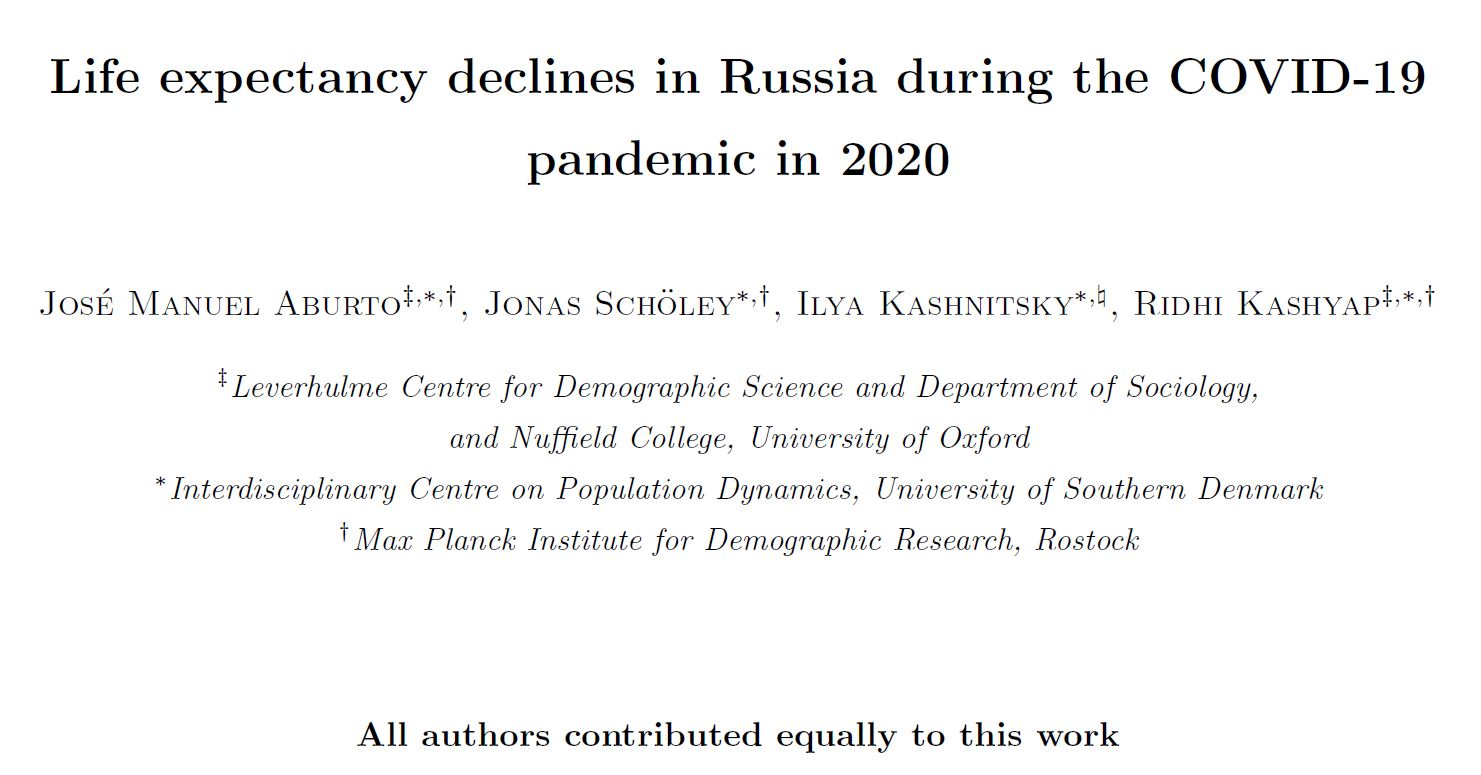
\includegraphics[scale=.6]{Figures/russia}		
		
	\end{center}
\end{frame}


\begin{frame}
	\LARGE{	
	\begin{center}
	
	\textbf{Russia}
	\hspace*{-1cm}
 \begin{tikzpicture}
\node (img) {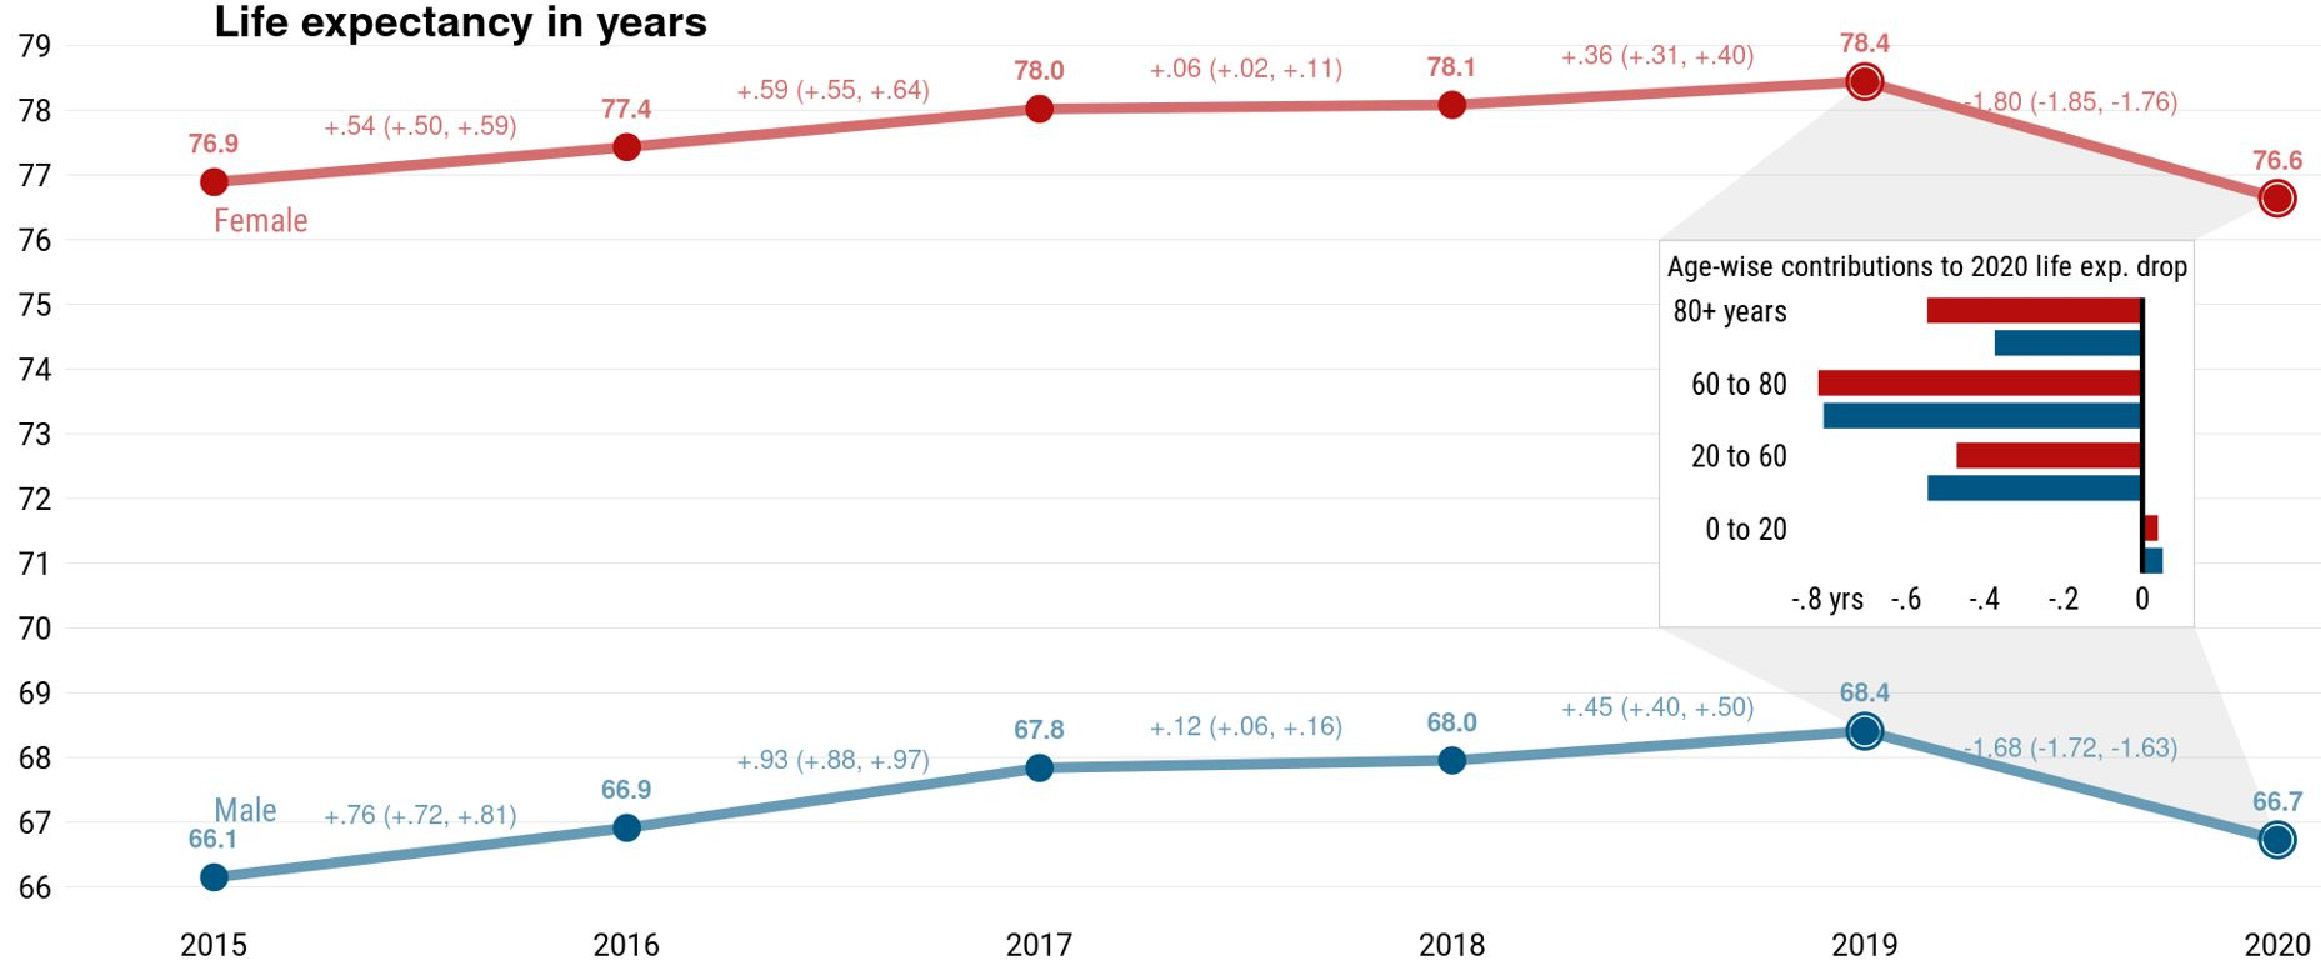
\includegraphics[width=1.13\textwidth]{Figures/Russia_1}};
\end{tikzpicture}
		
	\end{center}
		}
\end{frame}


\begin{frame}
	\LARGE{	
	\begin{center}
	
	\textbf{Russia}
	\hspace*{-1cm}
 \begin{tikzpicture}
\node (img) {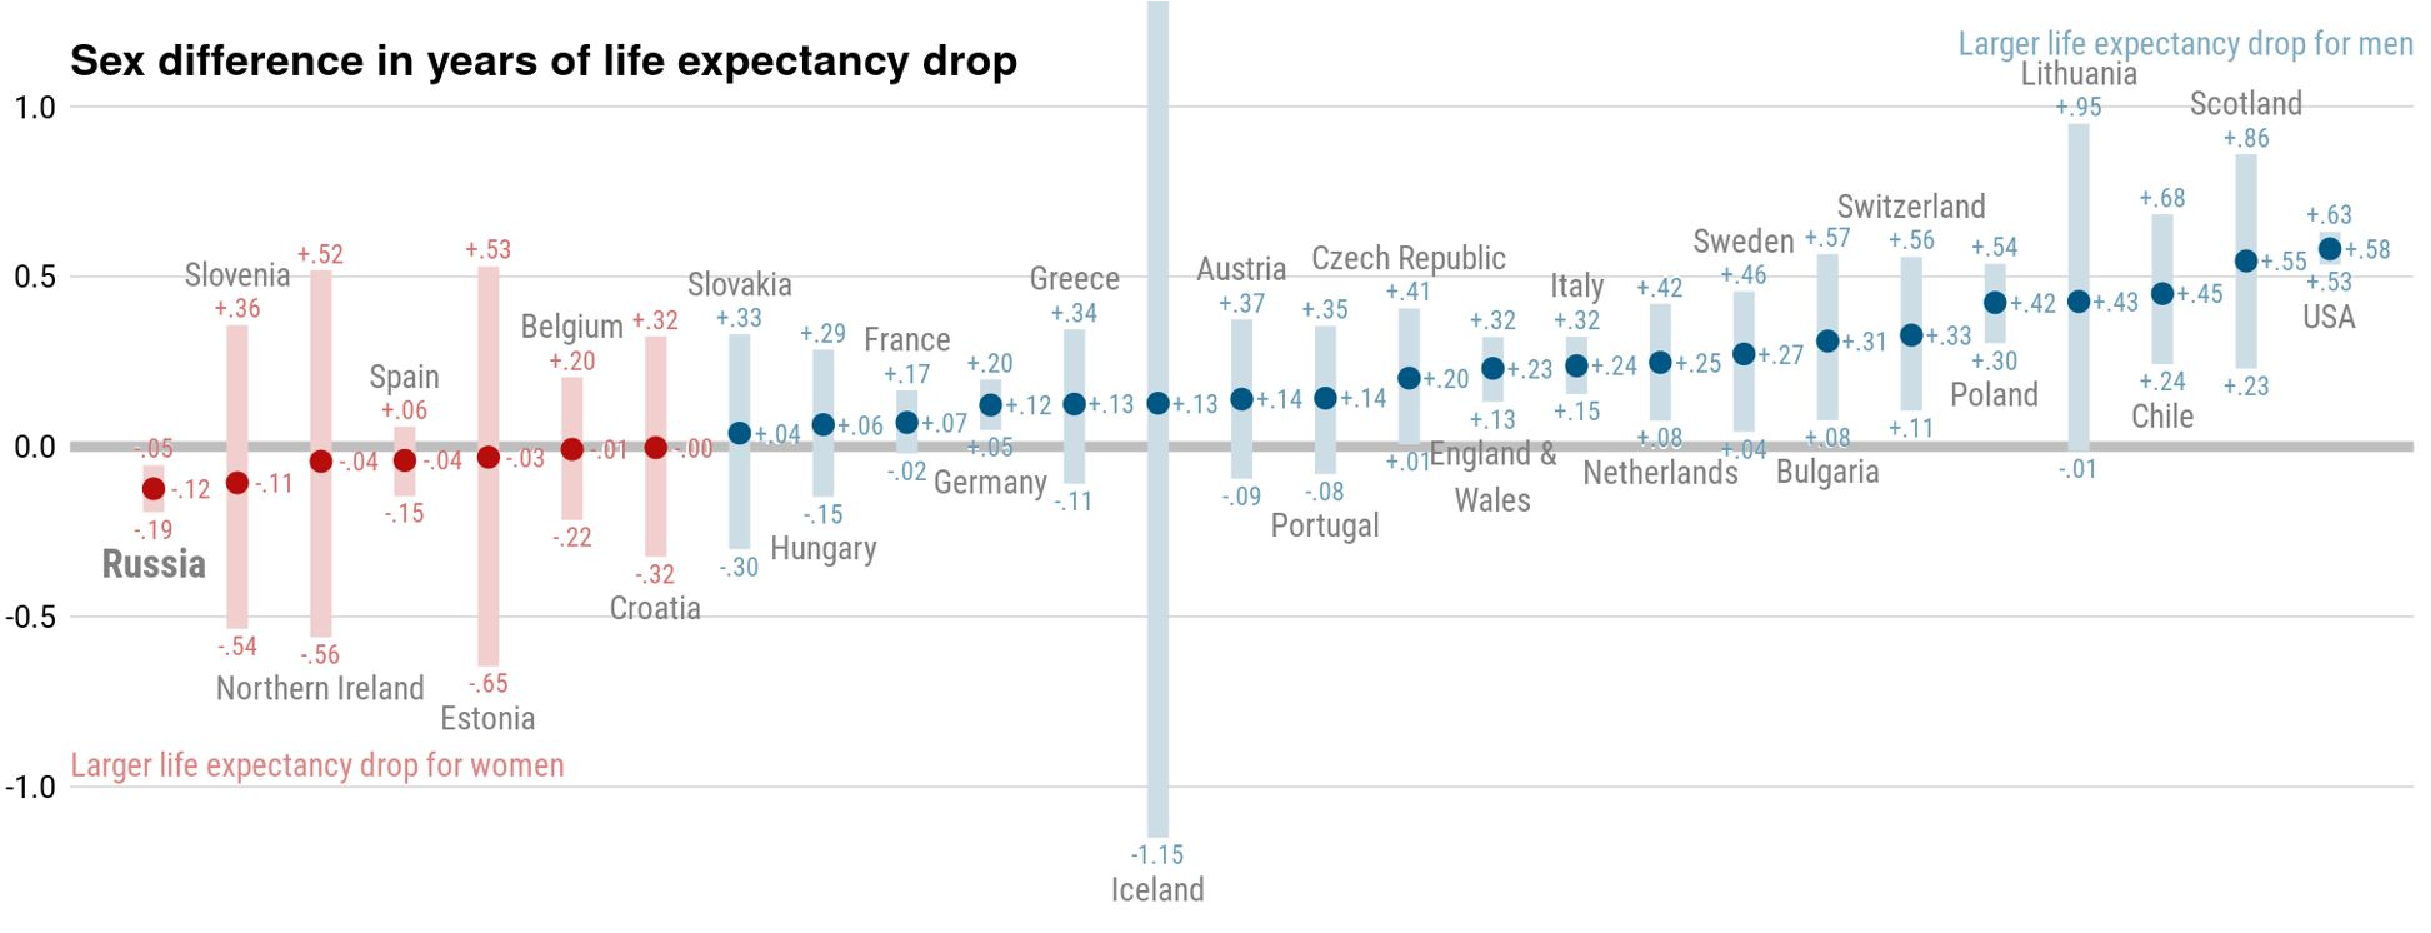
\includegraphics[width=1.13\textwidth]{Figures/Russia_2}};
\end{tikzpicture}
		
	\end{center}
		}
\end{frame}



\begin{frame}
	\begin{center}
	
			\LARGE{\textbf{Future prospects (short, medium, long term)}\linebreak \\ \pause
			
			\textbf{Subnational variation} \linebreak \\ \pause
			
			\textbf{Causes of death}}
		
	\end{center}
\end{frame}
%%%%%%%%%%%%%%%%%%%%%%%%%%%%%%%%%%%%%%%%%%%%%%%%%%%%%%%%%%%%%%%%%%%%%%%%

%%%%%%%%%%%%%%%%%%%%%%%%%%%%%%%%%%%%%%%%%%%%%%%%%%%%%%%%%%%%%%%%%%%%%%%%
\begin{frame}
 \begin{center}

			\color{black}\Large{\textbf{Jos\'{e} Manuel Aburto}}\\	
				
		\faEnvelope: jose-manuel.aburto@sociology.ox.ac.uk\\		
			\faTwitter \quad @jm\_aburto  @OxfordDemSci and @CPop\_SDU \\
			\faGithub \quad @jmaburto 
			$\,$\\
						$\,$\\
												\end{center}


\includegraphics[width=1 \textwidth,center]{Figures/logos}


 
 

\end{frame}

\end{document}
	

